\subsection{Design faults and problems}

\subsubsection{Membrane fragility}
As we previously touched on in paragraph \ref{sec: Design_of_the_membrane}, the membrane arms tend to \textbf{break} at the connection with the \textbf{cylindrical chamber}.
This is due to the abrupt change of profile that causes a stress concentration at that point.
This problem was especially noticeable during testing, as we had to \textbf{remove the magnet} from the chamber \textbf{multiple times} damaging the structure of the membrane.
Adding some fillets to the connection between the arms and the chamber helped to solve this problem, but it didn't eliminate it.
The good thing is that the membrane is \textbf{easily fixable} by adding very \textbf{small amounts of silicone} to the broken parts \textbf{as glue} and letting it cure.

\subsubsection{Overall system flexibility}
In the case of the small magnet, this design resulted in a \textbf{pretty flexible device} that could be bent a fair amount in all directions.
\begin{figure}[H]
    \centering
    \begin{subfigure}[b]{0.475\textwidth}
        \centering
        \includegraphics[width = 1\linewidth]{Chapters/Chapter5/Flexible_Mat_Prototypes/Figures/flexing_mat_top.png}
    \end{subfigure}
    \hfill
    \begin{subfigure}[b]{0.475\textwidth}  
        \centering 
        \includegraphics[width = 1\linewidth]{Chapters/Chapter5/Flexible_Mat_Prototypes/Figures/flexing_mat_btm.png}
    \end{subfigure}
    \caption{Flexible mat prototype bending.}
    \label{fig: Flexible_mat_bending}
\end{figure}

Meanwhile, in the case of the big magnet, the mat was also pretty flexible but the magnet with its size \textbf{impeded the structure from bending as much as the small magnet version}.

\subsubsection{Coil trap design faults}
The main problem with the coil trap design was that \textbf{screwing} the two parts together is not \textbf{reliable}.
As the two parts are connected by screws in only four points they tend to \textbf{separate when the mat is bent}.
This is because the lower part follows the bending of the mat through its fins, these fins are not directly connected to the upper part.

\begin{figure}[H]
    \centering
    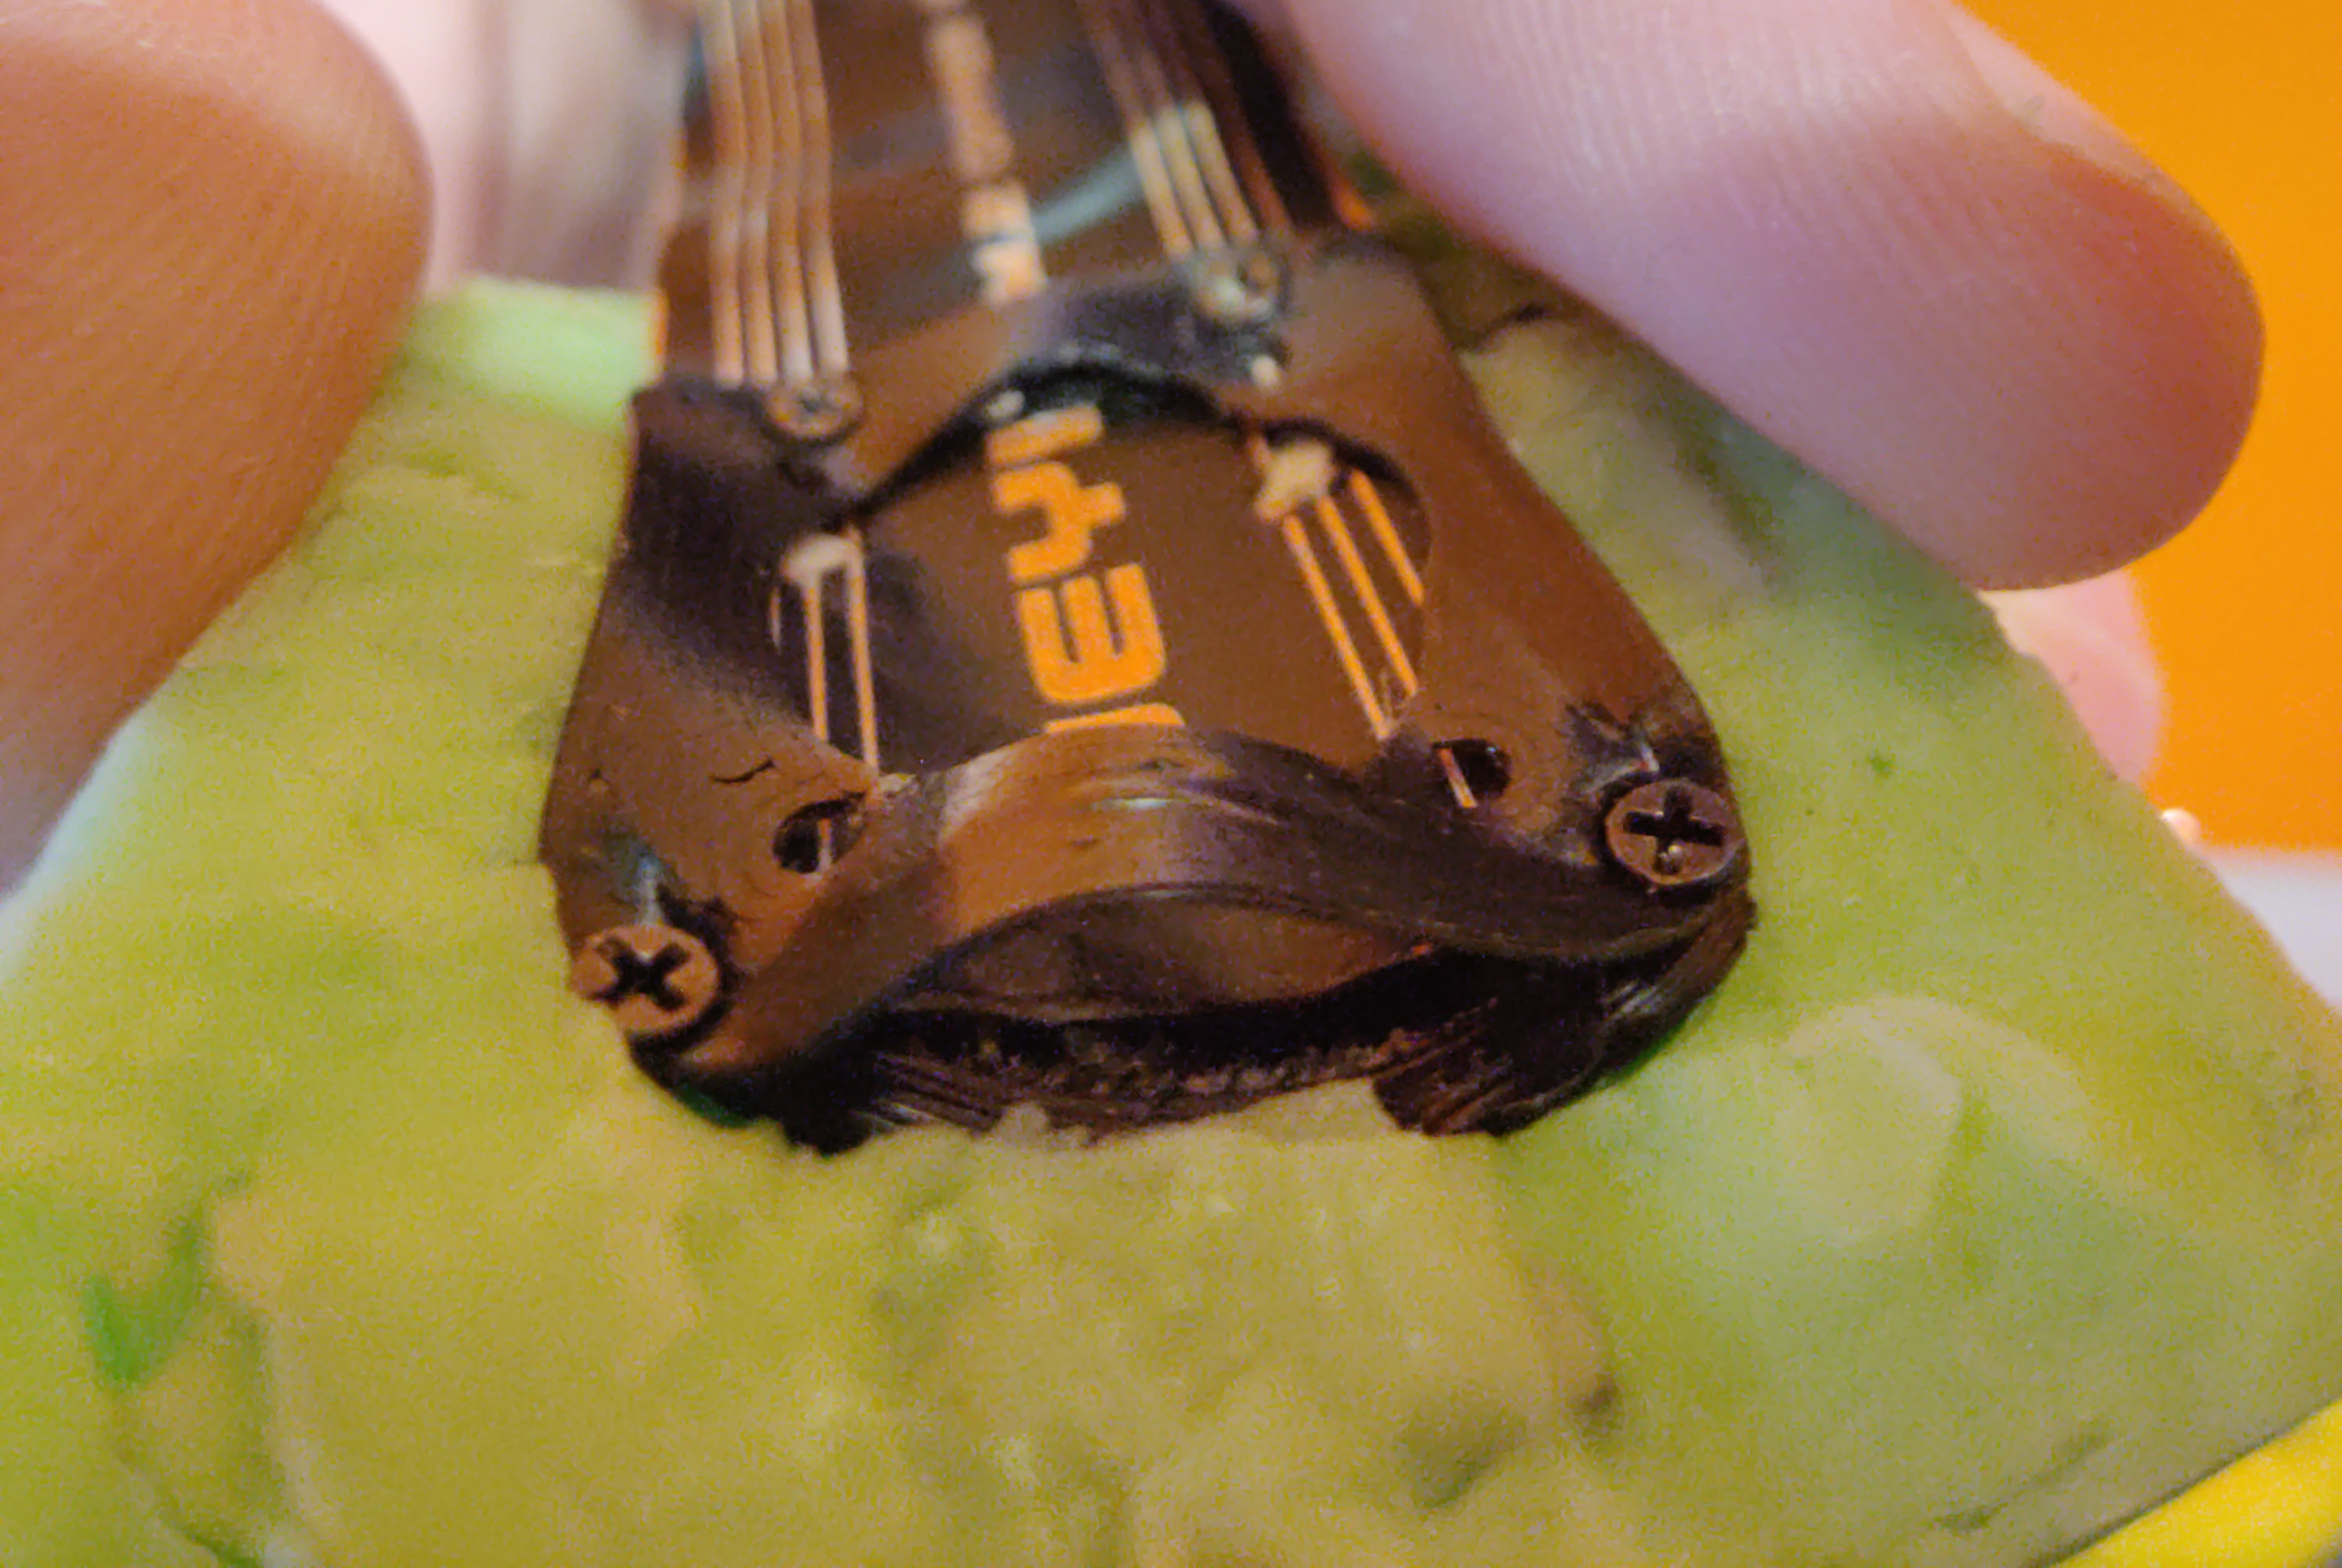
\includegraphics[width=0.7\linewidth]{Chapters/Chapter5/Flexible_Mat_Prototypes/Figures/coil_trap_separating.png}
    \caption{Coil trap separating when the mat is bent.}
    \label{fig: Coil_trap_separating}
\end{figure}